\documentclass[12pt,a4paper]{article}

\usepackage[utf8]{inputenc}
\usepackage[T1]{fontenc}
\usepackage[spanish]{babel}
\usepackage{geometry}
\usepackage{graphicx}
\usepackage{hyperref}
\usepackage{longtable}
\usepackage{float}
\usepackage{tikz}
\usepackage{array}
\usepackage{enumitem}
\usepackage{caption}
\usepackage[numbers]{natbib}
\usetikzlibrary{calc}

\geometry{margin=2.5cm}
\hypersetup{
    colorlinks=true,
    linkcolor=blue,
    urlcolor=blue,
    citecolor=blue
}

\begin{document}

\begin{titlepage}
\begin{tikzpicture}[remember picture, overlay]

    % Borde rojo exterior
    \draw[line width=2pt, red]
        ($(current page.north west)+(1cm,-1cm)$)
        rectangle
        ($(current page.south east)+(-1cm,1cm)$);

    % Borde verde interior
    \draw[line width=2pt, green!60!black]
        ($(current page.north west)+(1.5cm,-1.5cm)$)
        rectangle
        ($(current page.south east)+(-1.5cm,1.5cm)$);

\end{tikzpicture}

\begin{center}

{\Large \textbf{Universidad de las Fuerzas Armadas ESPE}}\\[0.5cm]

{\large Departamento de Ciencias de la Computación}\\[0.5cm]

{\normalsize Desarrollo de Aplicaciones Móviles}\\[0.5cm]

\begin{figure}[H]
    \centering
    
\includegraphics[width=0.5
    \linewidth]{img/escudo.png}
\end{figure} 


{\Large \textbf{Tarea 3.2: Desarrollo aplicaciones móviles con recursos remotos}}\\[0.8cm]

{\normalsize \textbf{NRC:} 30738 }\\[1cm]

{\large \textbf{Integrantes:}}\\[0.3cm]
Stefany Díaz\\
Jordy Viscaino\\
Jerson Llumiquinga\\
Moisés Benalcázar\\[1cm]

{\large \textbf{Docente:}}\\[0.3cm]
Ing. Doris Chicaiza\\[1cm]

{\large \textbf{Fecha:}}\\[0.3cm]
\today \\[1cm]

{\large \textbf{Marzo 2026 -- Agosto 2026}}

\end{center}

\end{titlepage}

\tableofcontents
\newpage
\listoffigures
\newpage

\section{Resumen}
Este informe presenta el desarrollo de una aplicación móvil construida en Flutter para gestionar contactos mediante operaciones básicas de creación, lectura, actualización y eliminación. La información se almacena localmente en una base de datos SQLite, mientras que el estado visual y de navegación se administra con Riverpod. Además, el proyecto incorpora validaciones de entrada, un tema visual configurable y una funcionalidad de llamada directa al contacto, lo que le da un alcance práctico y funcional \citep{flutter,sqlite,riverpod}.

\section{Introducción}
El desarrollo de aplicaciones móviles con almacenamiento local resulta útil cuando se requiere registrar información sin depender de servicios externos. En este proyecto se implementó una aplicación de contactos con una estructura clara, una interfaz sencilla y componentes reutilizables. La solución fue organizada por capas para separar la presentación, la lógica de negocio y el acceso a datos, con el fin de mantener el proyecto entendible y fácil de modificar \citep{flutter,sqlite}.

\section{Objetivos}
\subsection{Objetivo General}
Desarrollar una aplicación móvil en Flutter que permita gestionar contactos mediante operaciones CRUD, usando SQLite como mecanismo de persistencia local y Riverpod para la administración del estado.

\subsection{Objetivos Específicos}
\begin{itemize}[leftmargin=*]
    \item Implementar una interfaz sencilla para registrar y editar contactos.
    \item Guardar la información en una base de datos SQLite.
    \item Organizar el proyecto mediante una arquitectura por capas.
    \item Aplicar validaciones básicas sobre nombre, teléfono y correo.
    \item Incorporar una pantalla de configuración con modo oscuro persistente.
    \item Agregar una acción de llamada directa sobre el número almacenado.
\end{itemize}

\section{Marco Teórico}
\subsection{Flutter}
Flutter es un framework de Google para construir aplicaciones multiplataforma desde una sola base de código. Permite desarrollar interfaces consistentes para Android, iOS, web y escritorio con un rendimiento adecuado y una estructura de widgets flexible \citep{flutter}.

\subsection{SQLite}
SQLite es un motor de base de datos ligero que almacena la información en un archivo local. Es una opción práctica para aplicaciones móviles porque facilita el guardado de datos sin requerir servidor externo ni configuración compleja \citep{sqlite}.

\subsection{Riverpod}
Riverpod es una librería de administración de estado en Flutter. En este proyecto se usa para compartir datos entre la lógica y la interfaz, así como para controlar el modo oscuro, el listado de contactos y la selección de elementos en edición \citep{riverpod}.

\subsection{SharedPreferences}
SharedPreferences permite guardar datos simples de forma persistente en el dispositivo. En este proyecto se utiliza para conservar el estado del modo oscuro incluso después de cerrar y abrir nuevamente la aplicación \citep{sharedprefs}.

\subsection{Arquitectura por capas}
La arquitectura por capas divide el proyecto en partes como dominio, datos, aplicación y presentación. Esta organización mejora la lectura del código y facilita el mantenimiento, ya que cada capa cumple una responsabilidad específica.

\section{Desarrollo}
La aplicación fue construida con una estructura funcional y directa. Al abrirse, muestra una pantalla de bienvenida y luego dirige al usuario a una vista principal donde se encuentran las secciones de inicio, contactos y configuración. Desde ahí se pueden registrar contactos, revisar la lista almacenada, editar datos existentes, eliminarlos y ejecutar una llamada telefónica al número seleccionado.

\subsection{Estructura general del proyecto}
\begin{itemize}[leftmargin=*]
    \item \textbf{Dominio:} contiene la entidad \texttt{Contacto}, las interfaces del repositorio y servicios como validación y llamadas.
    \item \textbf{Aplicación:} contiene los casos de uso que agrupan las operaciones principales del CRUD.
    \item \textbf{Datos:} contiene el datasource local y la implementación del repositorio.
    \item \textbf{Presentación:} contiene pantallas, providers, helpers de interfaz y widgets reutilizables.
    \item \textbf{Temas:} contiene colores, estilos y configuración visual de la app.
\end{itemize}

\begin{figure}[H]
    \centering
    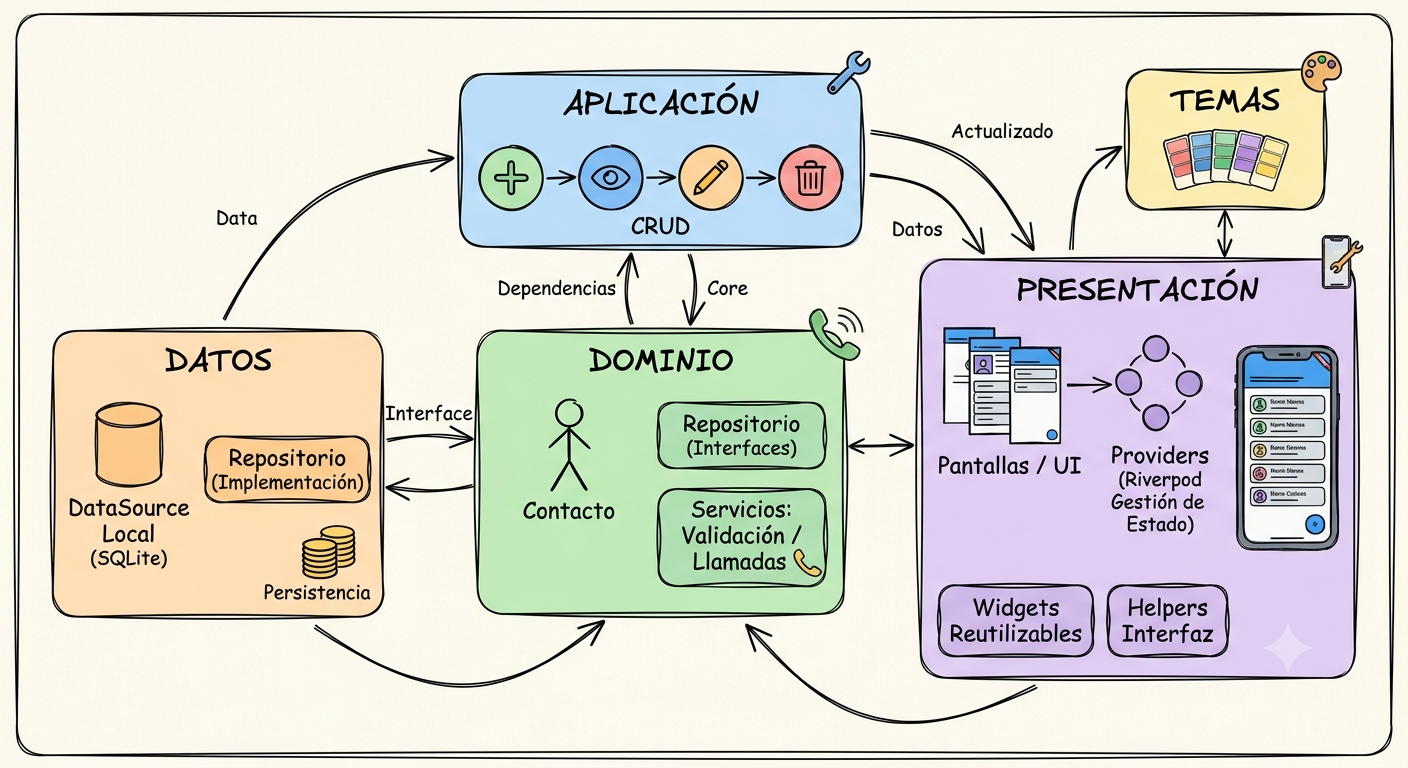
\includegraphics[width=0.8\textwidth]{img/estructura.png}
    \caption{Flujo de trabajo del proyecto.}
    \label{fig:estructura_proyecto}
\end{figure}

% Figura sugerida:
% Captura del árbol de carpetas o diagrama de arquitectura por capas del proyecto.

\subsection{Inicio de la aplicación}
El punto de entrada se encuentra en \texttt{main.dart}. Allí se inicializa la base de datos SQLite antes de mostrar la interfaz principal. Luego, la aplicación se envuelve en un \texttt{ProviderScope} para exponer el estado global a las pantallas. La primera vista que se carga es la pantalla de bienvenida, la cual muestra el logo institucional durante unos segundos antes de redirigir al menú principal.

% Figura sugerida:
% Captura de \texttt{main.dart} y captura de la pantalla splash.
    
\begin{figure}[H]
    \centering
    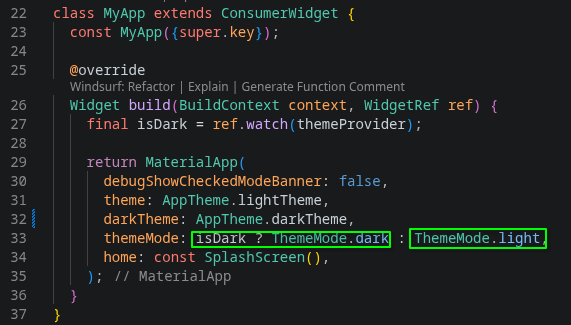
\includegraphics[width=0.8\textwidth]{img/main.png}
    \caption{Clase MyApp.}
    \label{fig:splash}
\end{figure}

\begin{figure}[H]
    \centering
    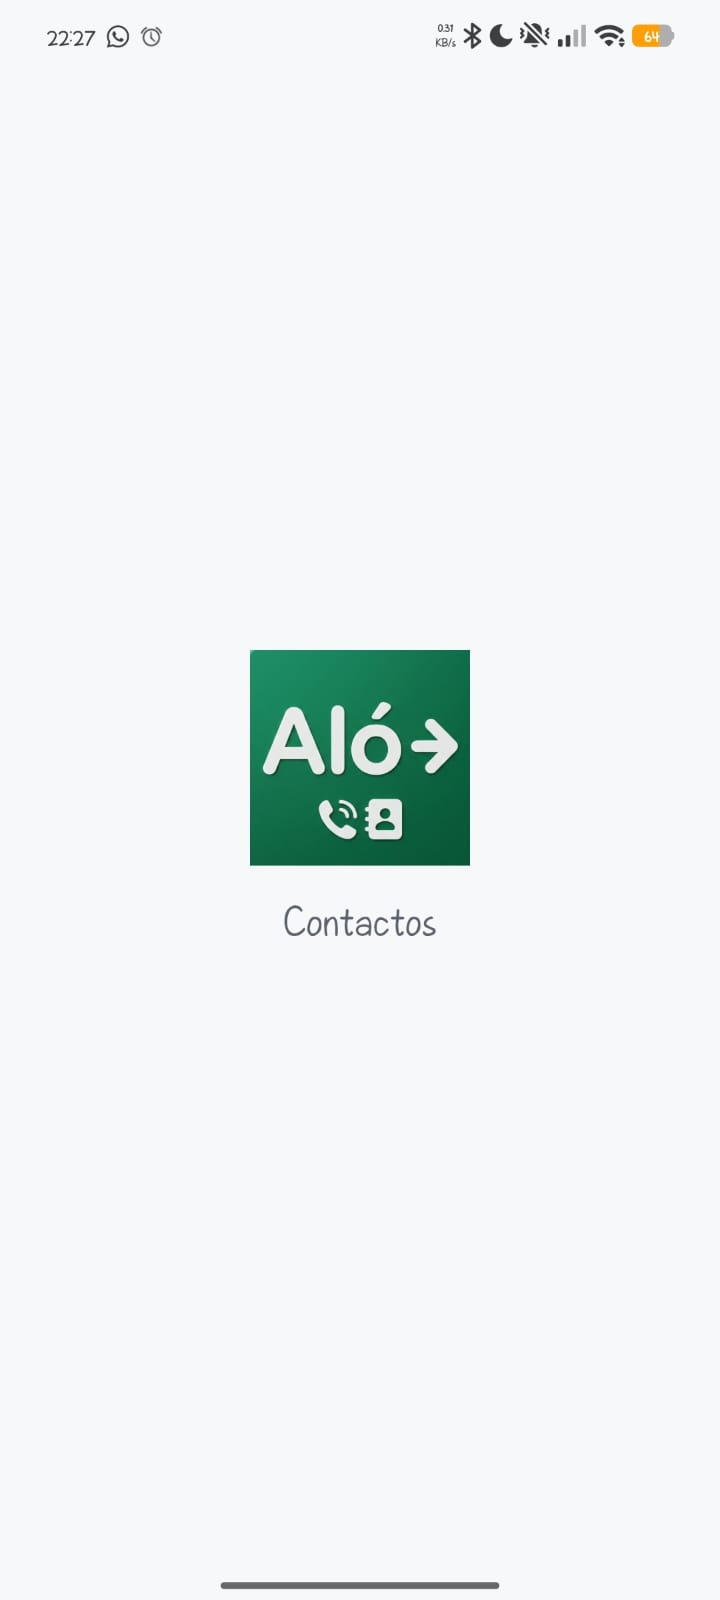
\includegraphics[width=0.5\textwidth]{img/splash.png}
    \caption{Pantalla de bienvenida.}
    \label{fig:splash}
\end{figure}

\subsection{Pantalla principal}
La pantalla principal está dividida en tres secciones mediante una barra inferior de navegación. La primera corresponde al formulario de registro, la segunda a la lista de contactos y la tercera a la configuración. Esta distribución permite mantener el flujo de uso claro y evita mezclar demasiadas acciones en una sola vista.

% Figura sugerida:
% Captura del menú principal con la barra inferior de navegación.

\begin{figure}[H]
    \centering
    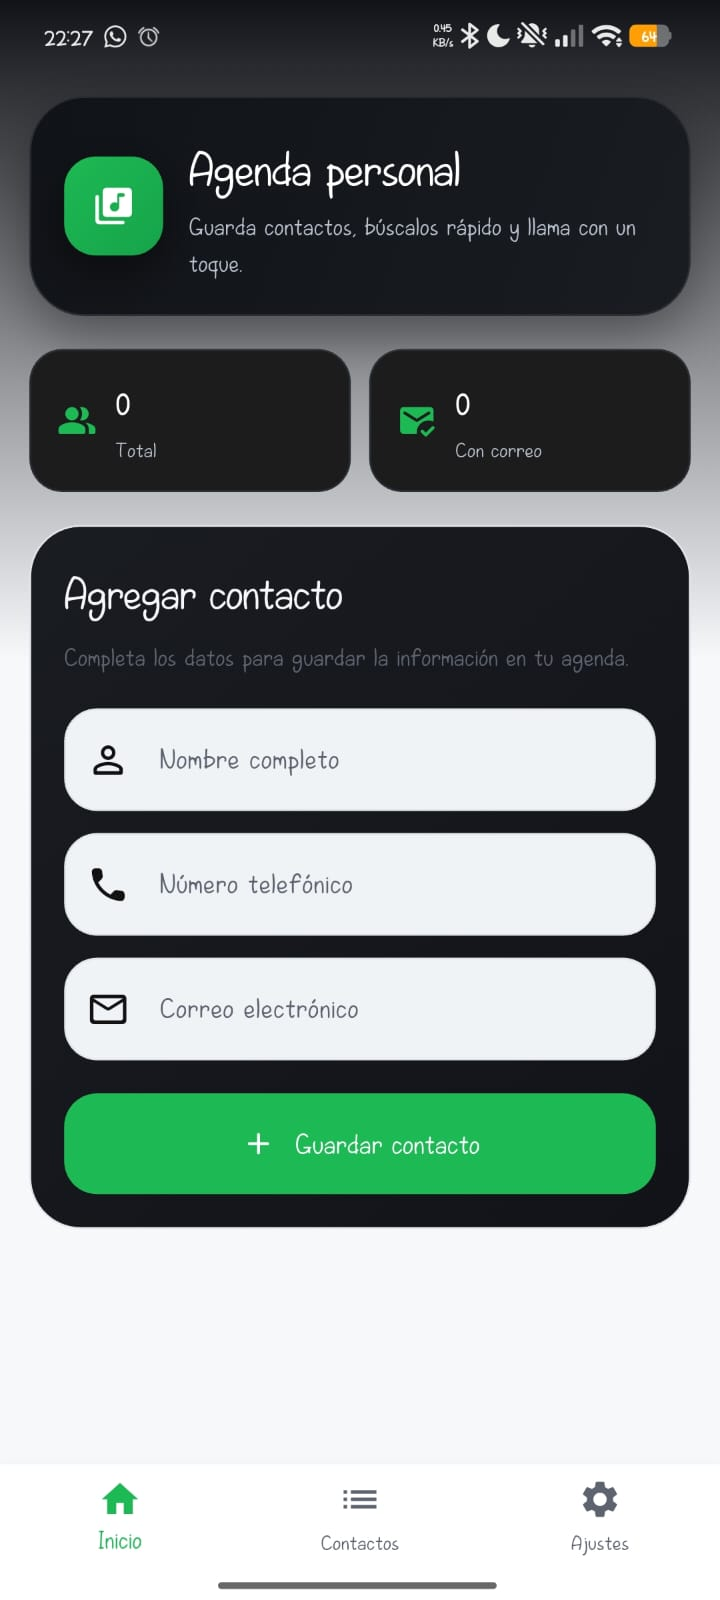
\includegraphics[width=0.5\textwidth]{img/home.png}
    \caption{Pantalla principal.}
    \label{fig:menu}
\end{figure}


\subsection{Registro y validación de contactos}
En la sección de inicio se ingresan nombre, teléfono y correo. Antes de guardar, el sistema valida que el nombre no esté vacío ni contenga números, que el teléfono tenga 10 dígitos y que el correo tenga un formato válido. Si alguna validación falla, se muestra un mensaje breve en pantalla mediante un snackbar.

\begin{figure}[H]
    \centering
    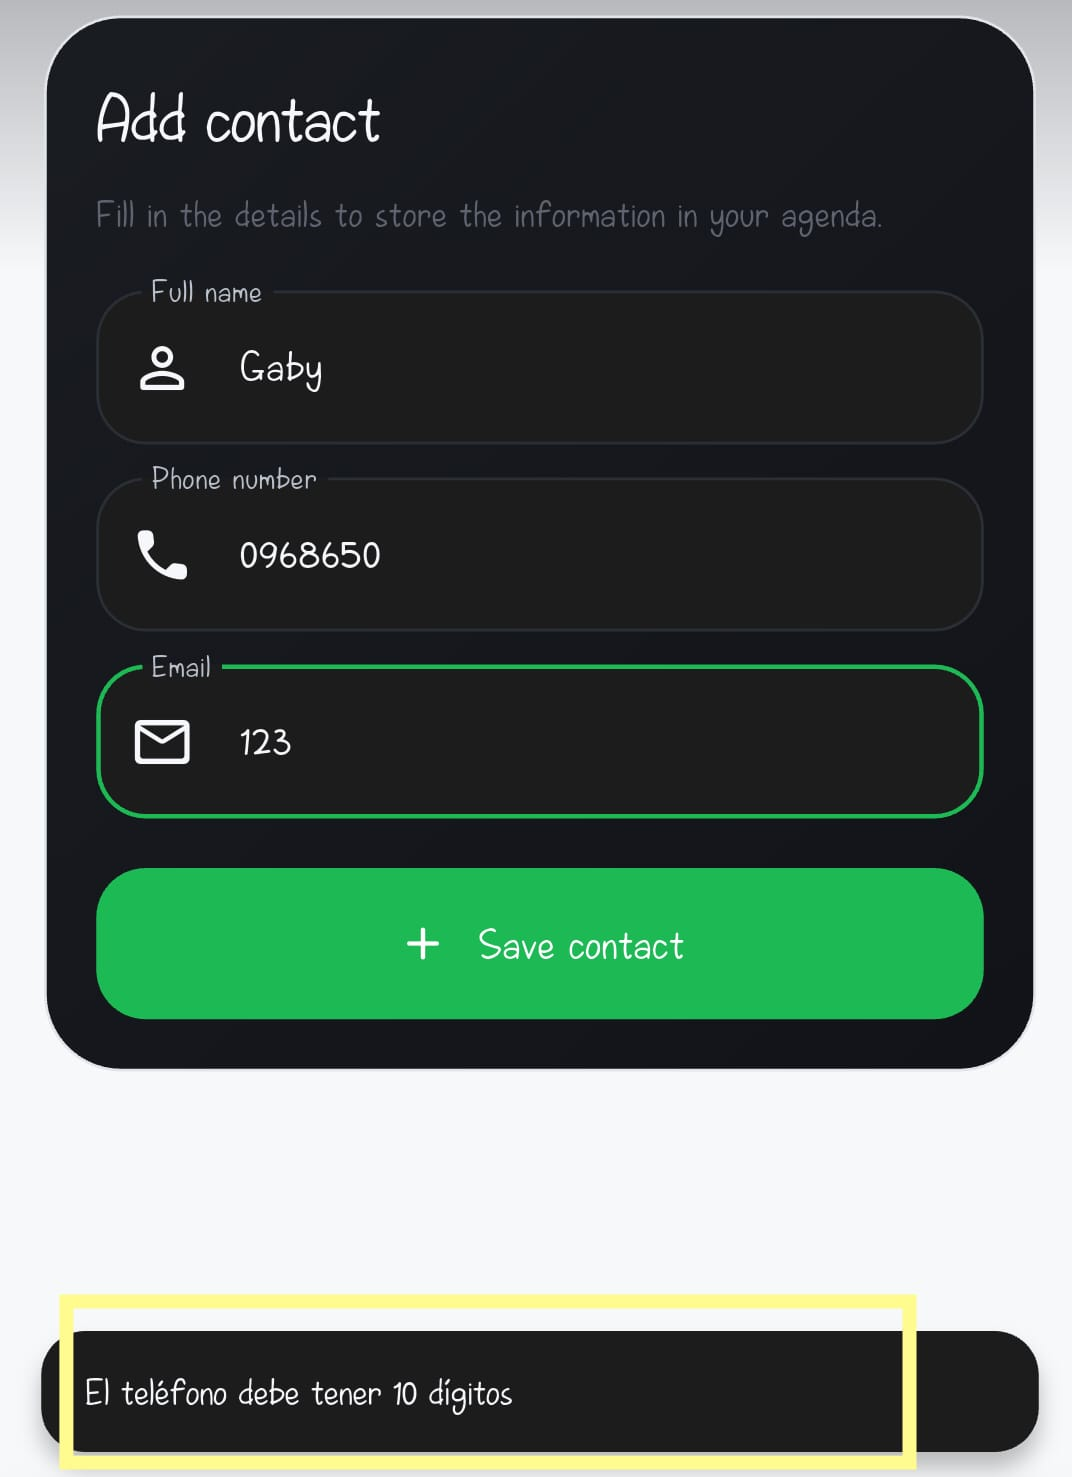
\includegraphics[width=0.8\textwidth]{img/numincorrecto.png}
    \caption{Formulario de registro de contactos con validación.}
    \label{fig:formulario}
\end{figure}

\begin{figure}[H]
    \centering
    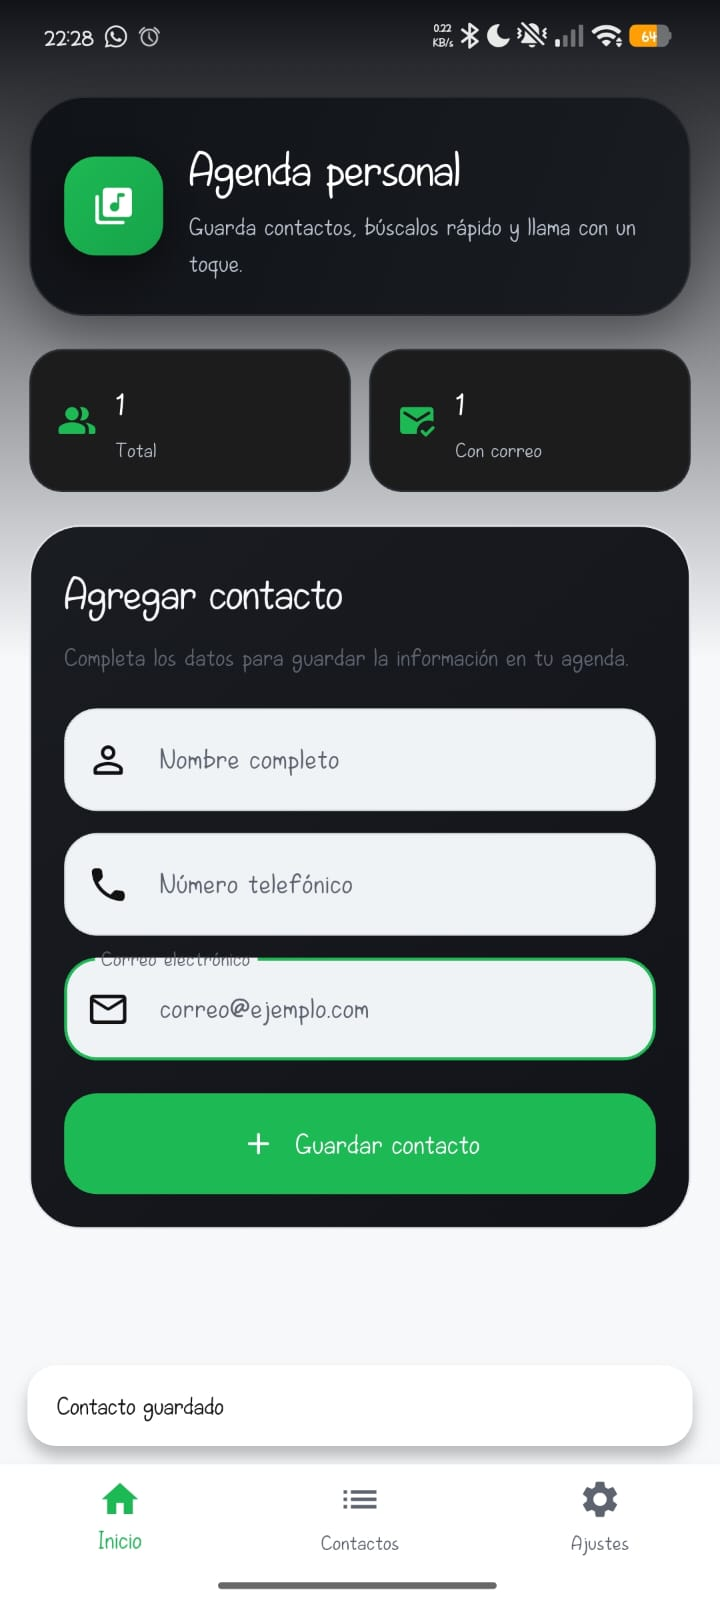
\includegraphics[width=0.5\textwidth]{img/guardado.png}
    \caption{Registro de contacto exitoso.}
    \label{fig:formulario}
\end{figure}

% Figura sugerida:
% Captura del formulario con un mensaje de validación visible.
% Captura del formulario ya diligenciado con datos correctos.

\subsection{Listado, edición y eliminación}
La sección de contactos muestra todos los registros almacenados. Cada elemento presenta acciones para llamar, editar o eliminar. Al editar, se abre una vista específica que carga los datos del contacto y permite actualizarlos. Al eliminar, el registro se borra de la base local y la lista se refresca automáticamente.

% Figura sugerida:
% Captura de la lista de contactos con botones de llamar, editar y eliminar.
% Captura de la pantalla de edición de un contacto.

\begin{figure}[H]
    \centering
    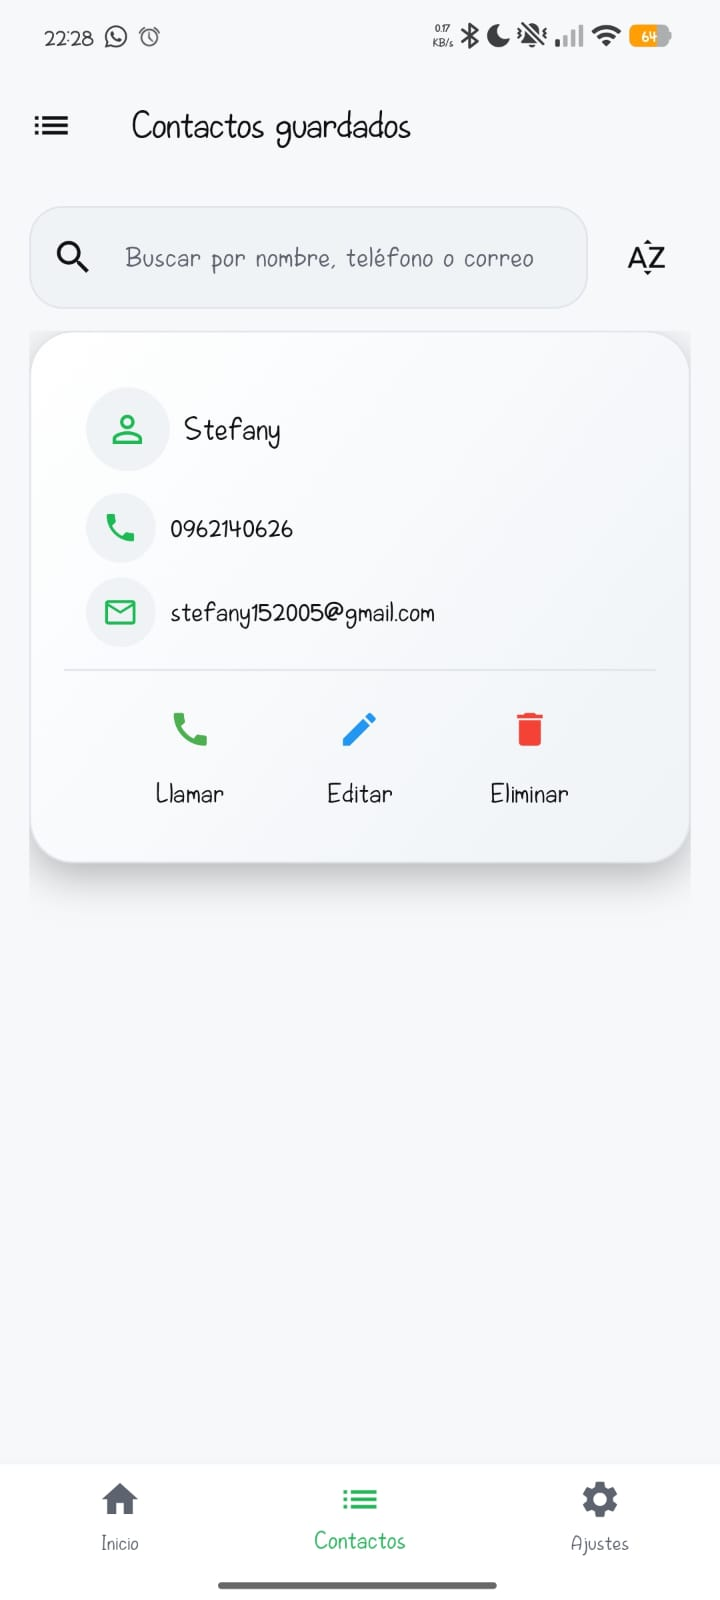
\includegraphics[width=0.5\textwidth]{img/lista.png}
    \caption{Lista de contactos con acciones de editar, llamar y eliminar.}
    \label{fig:lista}
\end{figure}

\subsection{Configuración visual}
La pantalla de configuración contiene un interruptor para activar o desactivar el modo oscuro. El estado se guarda de manera persistente usando \texttt{SharedPreferences}, de modo que la preferencia del usuario se conserva aunque la aplicación se cierre. Tambien se agrego un switch para cambiar el idioma de la aplicacion, el cual se encuentra en ingles y español.

% Figura sugerida:
% Captura de la pantalla de configuración con el switch de modo oscuro.

\begin{figure}[H]
    \centering
    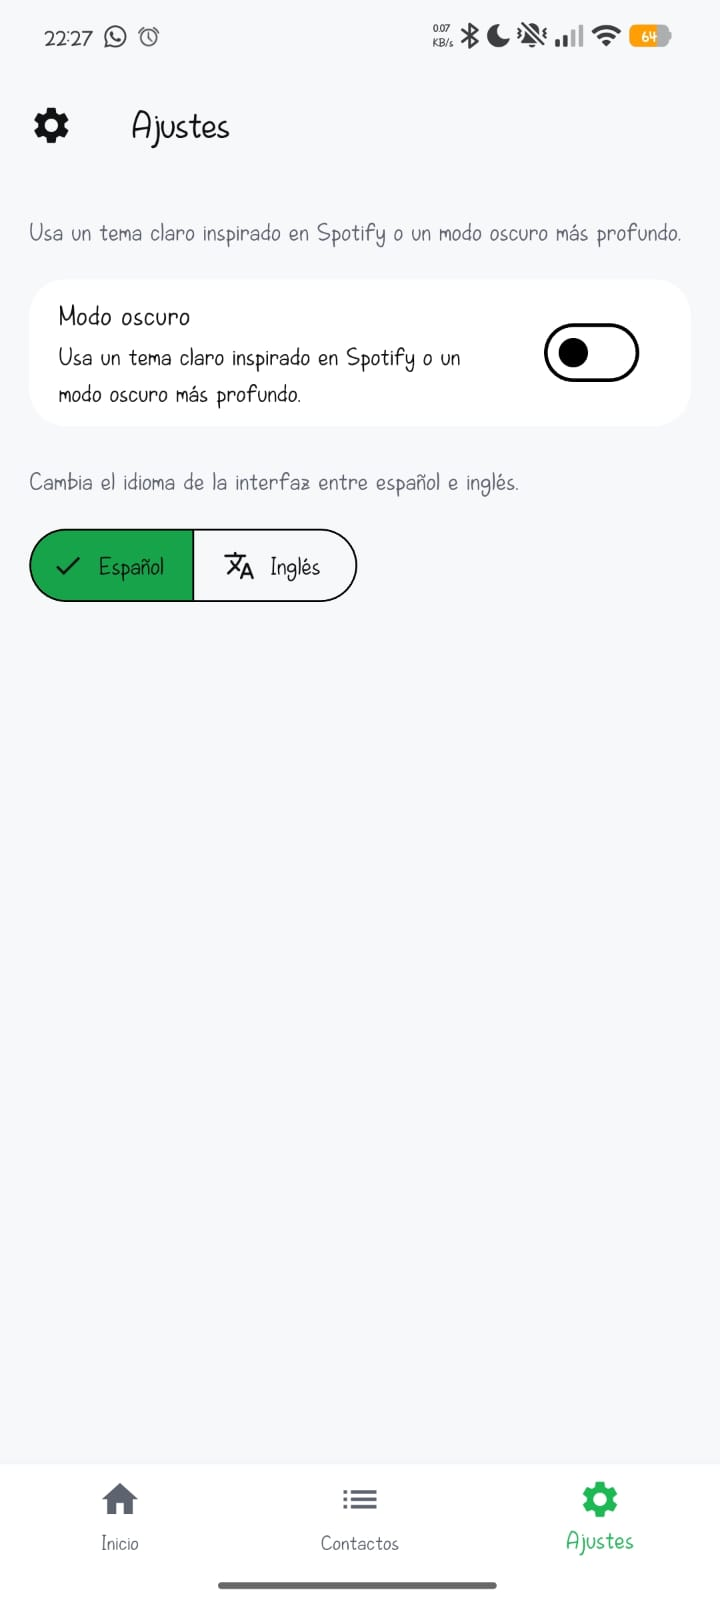
\includegraphics[width=0.5\textwidth]{img/modoclaro.png}
    \caption{Pantalla de configuración con modo claro e idioma español.}
    \label{fig:configuracion}
\end{figure}      


\begin{figure}[H]
    \centering
    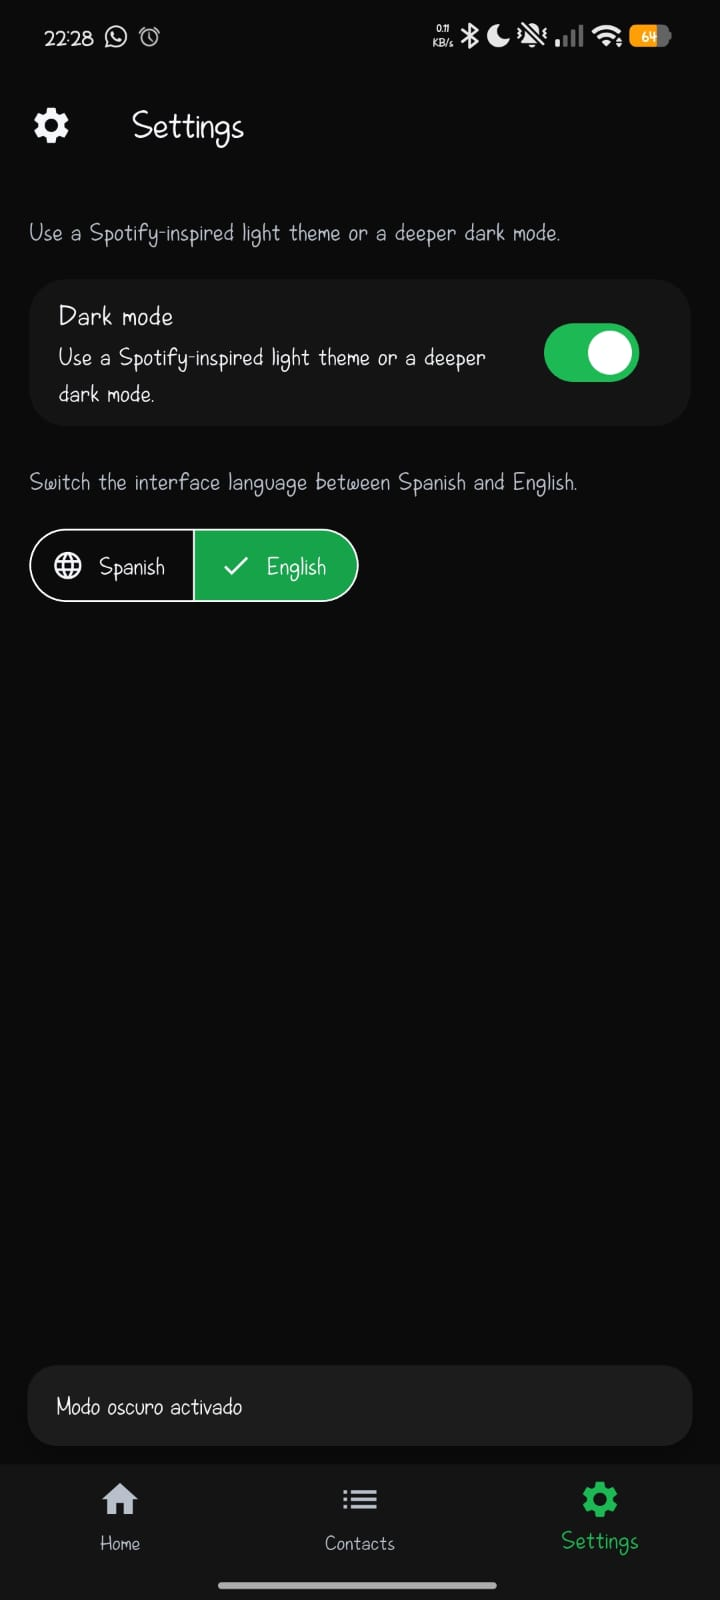
\includegraphics[width=0.5\textwidth]{img/modooscuro.png}
    \caption{Pantalla de configuración con modo oscuro e idioma inglés.}
    \label{fig:configuracion}
\end{figure}      



\subsection{Persistencia de datos}
La base de datos se crea con una tabla llamada \texttt{contactos}. Esta tabla almacena un identificador, nombre, teléfono y correo. El datasource local se encarga de ejecutar las operaciones de insertar, consultar, actualizar y eliminar, mientras que el repositorio sirve como intermediario entre la lógica y el acceso a datos.

% Figura sugerida:
% Captura del archivo sqlite_service.dart o del esquema de la tabla contactos.

\begin{figure}[H]
    \centering
    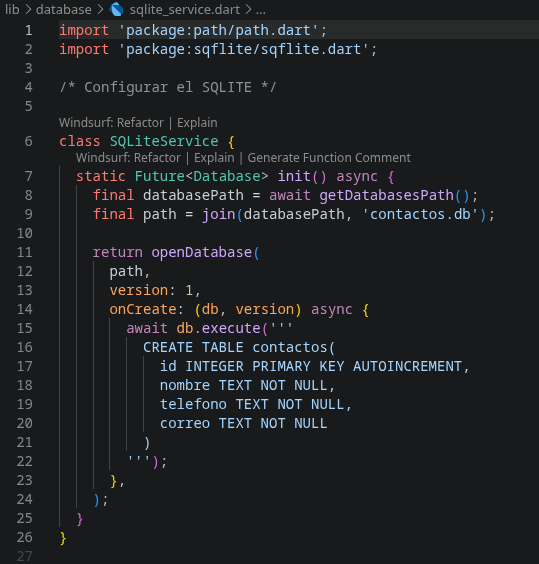
\includegraphics[width=0.8\textwidth]{img/sqlite.png}
    \caption{Esquema de la tabla contactos en SQLite.}
    \label{fig:sqlite}
\end{figure}  

\subsection{Funcionalidad de llamada}
La aplicación incluye la posibilidad de llamar directamente al número guardado. Para ello se solicita el permiso telefónico, se normaliza el número y se ejecuta la llamada usando el servicio correspondiente. Esta función agrega un valor práctico a la aplicación, ya que permite usar el contacto sin salir de la interfaz.

% Figura sugerida:
% Captura del código del servicio de llamada o de la acción sobre un contacto.

\begin{figure}[H]
    \centering
    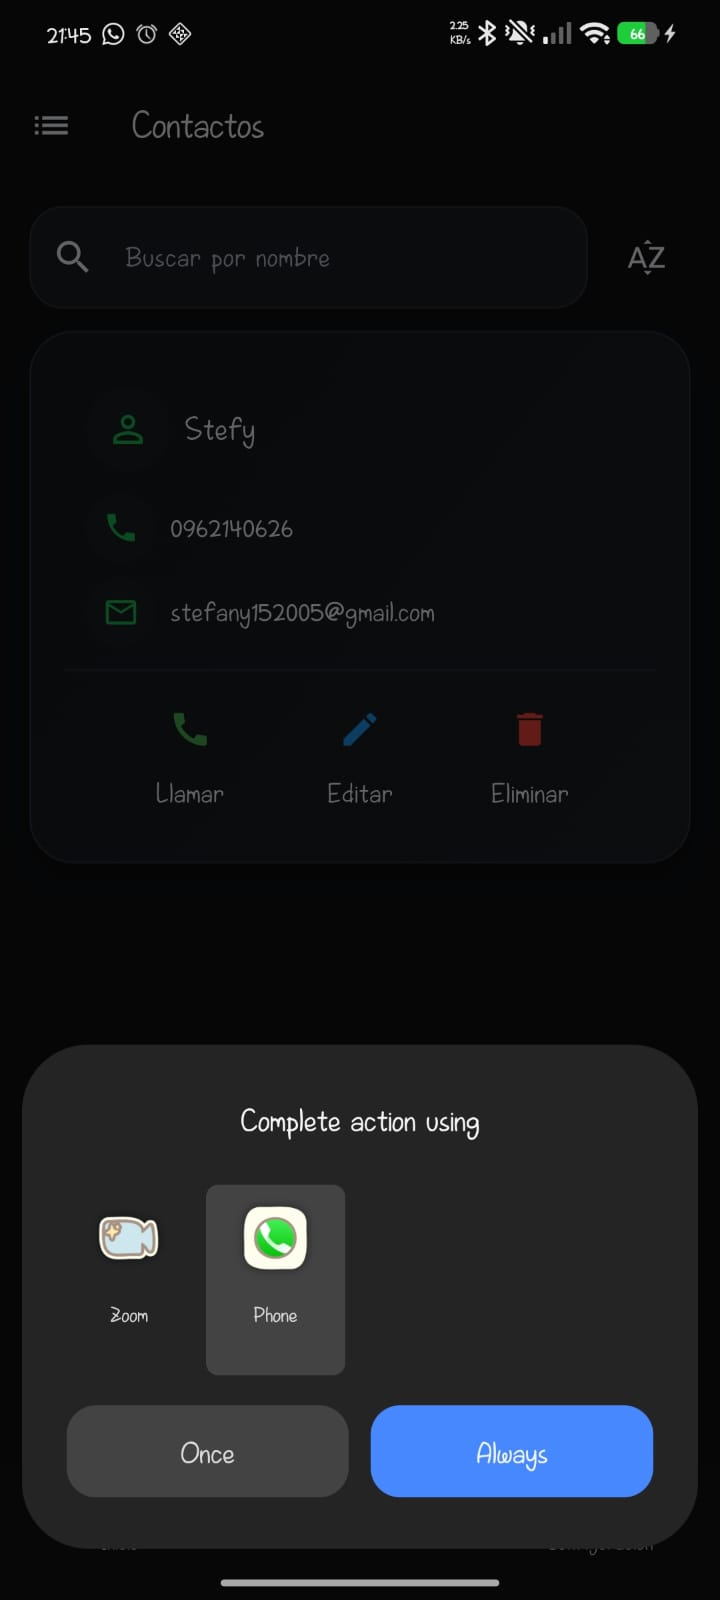
\includegraphics[width=0.5\textwidth]{img/llamada.png}
    \caption{Funcionalidad de llamada.}
    \label{fig:llamada}
\end{figure} 

\subsection{Estructura de carpetas}
\begin{longtable}{|p{0.30\textwidth}|p{0.62\textwidth}|}
\hline
\textbf{Carpeta} & \textbf{Descripción} \\
\hline
\texttt{lib/main.dart} & Punto de entrada de la aplicación. \\
\hline
\texttt{lib/domain} & Entidades, contratos y servicios de dominio. \\
\hline
\texttt{lib/application} & Casos de uso de la lógica principal. \\
\hline
\texttt{lib/data} & Datasource local y repositorio. \\
\hline
\texttt{lib/presentation} & Pantallas, providers y utilidades de interfaz. \\
\hline
\texttt{lib/widgets} & Componentes visuales reutilizables. \\
\hline
\texttt{lib/themes} & Colores, estilos y configuración visual. \\
\hline
\texttt{assets/images} & Recursos gráficos de la aplicación. \\
\hline
\end{longtable}

\section{Conclusiones}
Se desarrolló una aplicación móvil sencilla y funcional para gestionar contactos. La combinación de Flutter, SQLite y Riverpod permitió construir una solución ordenada, persistente y fácil de mantener. Además, el proyecto incluye elementos adicionales como validación de datos, modo oscuro y llamadas telefónicas, lo que mejora la utilidad general de la aplicación. La estructura por capas facilitó una organización clara del código y deja una base adecuada para futuras mejoras.

\section{Referencias}
\bibliographystyle{plainnat}
\bibliography{ref}

\end{document}
